\section{CLUE3D performance with pileup}
\label{sec:pileup}

Pileup introduces many nearby showers with a broad range of energies and
particle species. I studied samples with an average of 200 additional interactions per bunch
crossing (PU200), keeping two efficiencies apart: the efficiency of
reconstructing the injected signal photon, and the inclusive efficiency
measured over all selected in-time SimTracksters (signal plus pileup). This distinction is essential:
the signal-only curve tests the same displaced-photon topology in a busier
environment, whereas the inclusive curve also changes the population being
measured.

\subsection{Signal efficiency and the meaning of displacement}

\begin{figure}[!htbp]
  \centering
  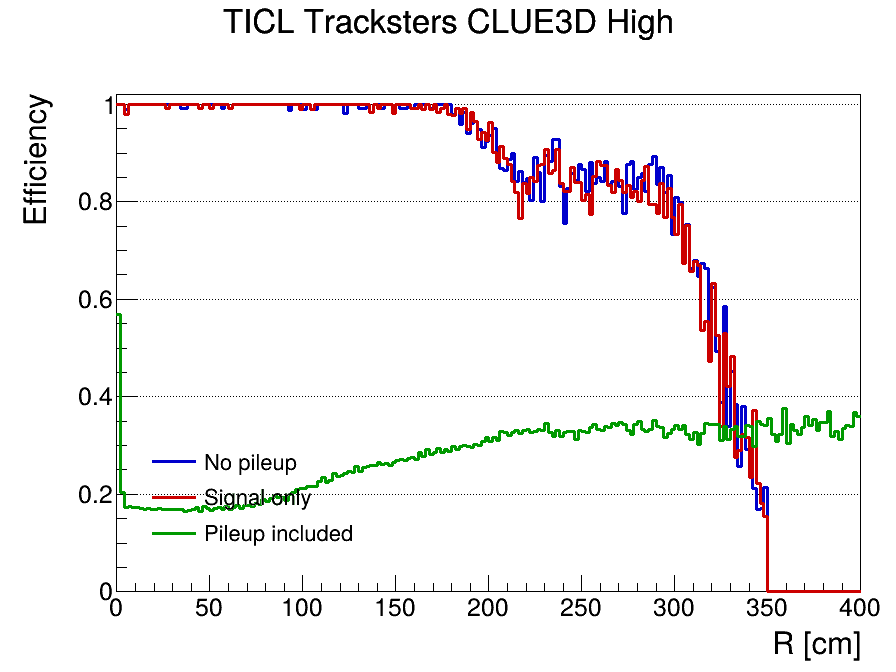
\includegraphics[width=\linewidth]{figures/pileup_efficiency.png}
  \caption{Default \cluethreed{} efficiency without pileup, for the generated
  signal photon in PU200, and for the inclusive in-time truth selection in
  PU200. The inclusive curve has a different denominator and a different
  interpretation of resolved $\R$ for charged particles.}
  \label{fig:pileupefficiency}
\end{figure}

Figure~\ref{fig:pileupefficiency} compares the no-pileup photon sample, the
signal photon in PU200, and the inclusive PU200 selection. The first two
curves are similar: both retain high efficiency at small displacement and
show the large-$\R$ degradation identified in
Section~\ref{sec:singlephoton}. The inclusive curve is quite different, and it
is dominated by pileup: the signal photon accounts for fewer than $1$ in
$1000$ of the selected in-time SimTracksters, so the inclusive denominator is
essentially the pileup population rather than the injected photon. It
falls sharply just outside the first displacement bin, reaches a minimum,
and then increases over a broad range of $\R$. This shape cannot be read as
the response to a single photon displaced progressively farther from the
beamline. A comparison of the Trackster and TICL-candidate efficiencies also
showed no substantial change in this behaviour at the candidate stage.

For pileup particles, resolved $\R$ is particularly easy to misinterpret. The
boundary position and direction define a line that can be extrapolated to
$z=0$. Charged particles bend in the magnetic field, so this line is a tangent
to a curved trajectory. Its intercept can be far from the beamline even when
the particle was produced close to it. A large resolved $\R$ in pileup is
therefore not evidence for a physically displaced production vertex. The
reconstruction consequences, however, are the same either way: a trajectory
with a large intercept still projects poorly onto the interaction point, so by
Eq.~\eqref{eq:displacedscale} its LayerClusters are pushed apart as
$d_{XY}\simeq\R|\Delta z|/z$ and suffer the same fragmentation as a genuinely
displaced shower.

Even for a straight photon trajectory, the longitudinal spread of collision
vertices matters. For a photon produced on the beamline at $z=z_v$, the
transverse intercept of its line at $z=0$ has magnitude
\begin{equation}
 R=|z_v|\tan\theta,
 \label{eq:pileupphotonR}
\end{equation}
where $\theta$ is the momentum polar angle relative to the beam axis, taking
the corresponding acute angle in either endcap. It is not the same experiment as
varying the transverse production offset of the displaced gun.

\subsection{Separating particle composition from reconstruction effects}

To investigate the inclusive shape, I broke the efficiency down per particle
in a 20\,000-event study, so that numerator and denominator could be examined
in the same kinematic slices.

\begin{figure*}[!tp]
  \centering
  \begin{subfigure}{0.49\textwidth}
    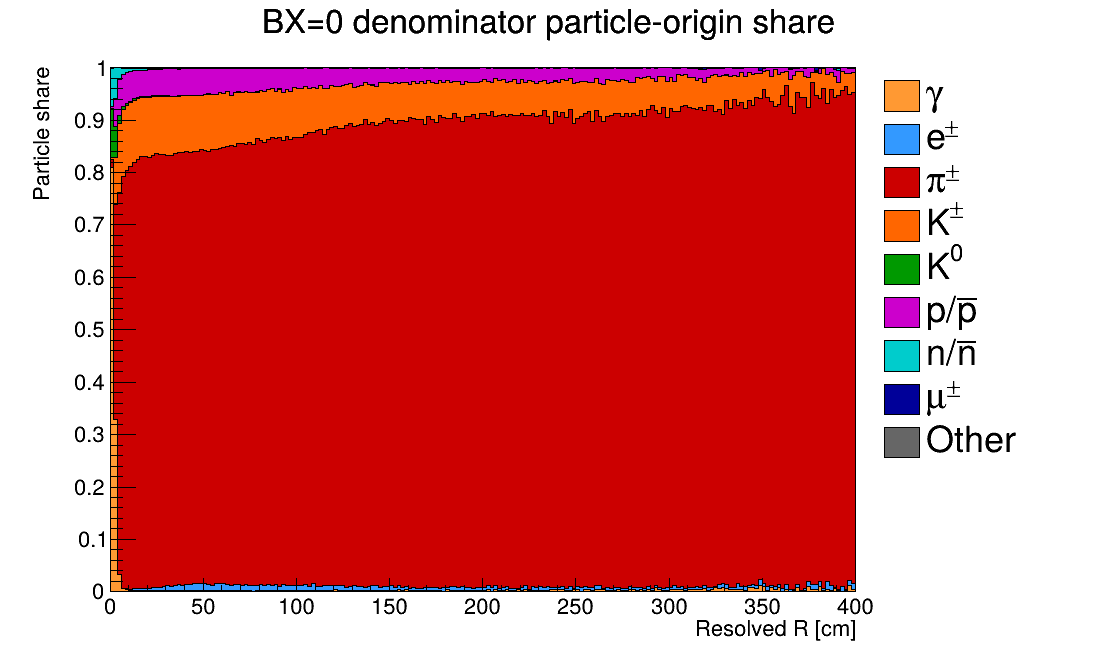
\includegraphics[width=\linewidth]{figures/pileup_composition.png}
    \caption{Composition of the in-time truth denominator.}
  \end{subfigure}\hfill
  \begin{subfigure}{0.49\textwidth}
    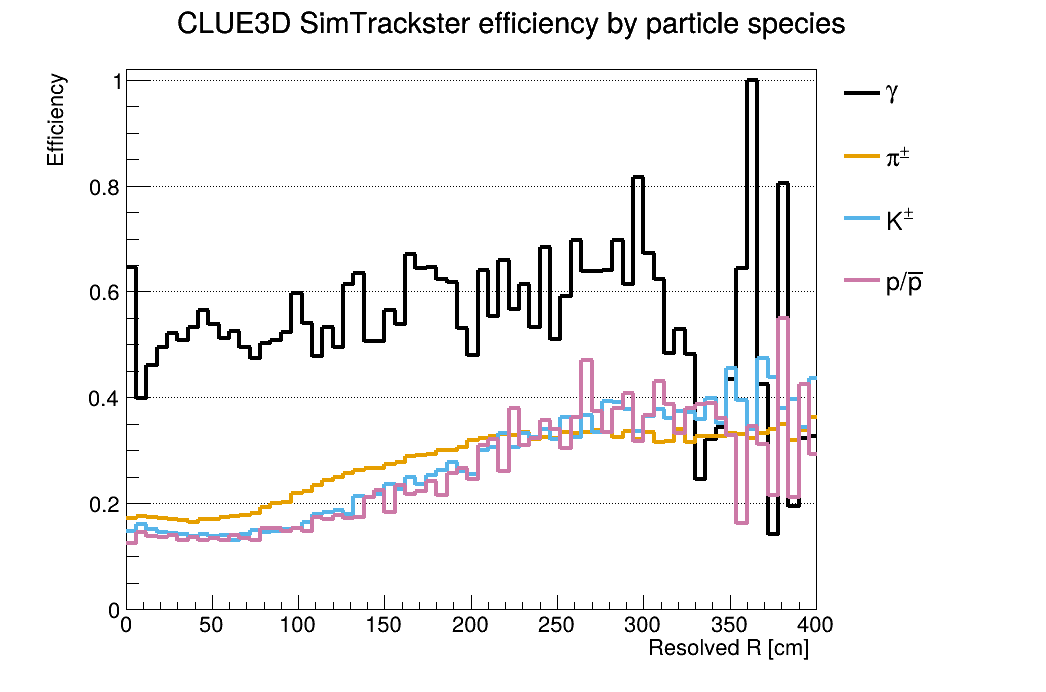
\includegraphics[width=\linewidth]{figures/pileup_efficiency_pid.png}
    \caption{Efficiency split by particle species.}
  \end{subfigure}
  \caption{Particle composition and reconstruction efficiency versus resolved
  $\R$ in pileup. The changing mixture contributes to the inclusive curve,
  but does not explain the displacement dependence within each species.}
  \label{fig:pileuppid}
\end{figure*}

The truth composition changes rapidly near $\R=0$. Photons contribute
strongly in the first bins, while charged pions dominate most of the larger
resolved-displacement range (Fig.~\ref{fig:pileuppid}). This accounts for part
of the inclusive change, but it is not a complete explanation: efficiencies
within individual species still depend on $\R$. Photon efficiency falls,
whereas the charged-hadron curves tend to rise. The remaining investigation
therefore treats these populations separately.

\begin{figure}[!htbp]
  \centering
  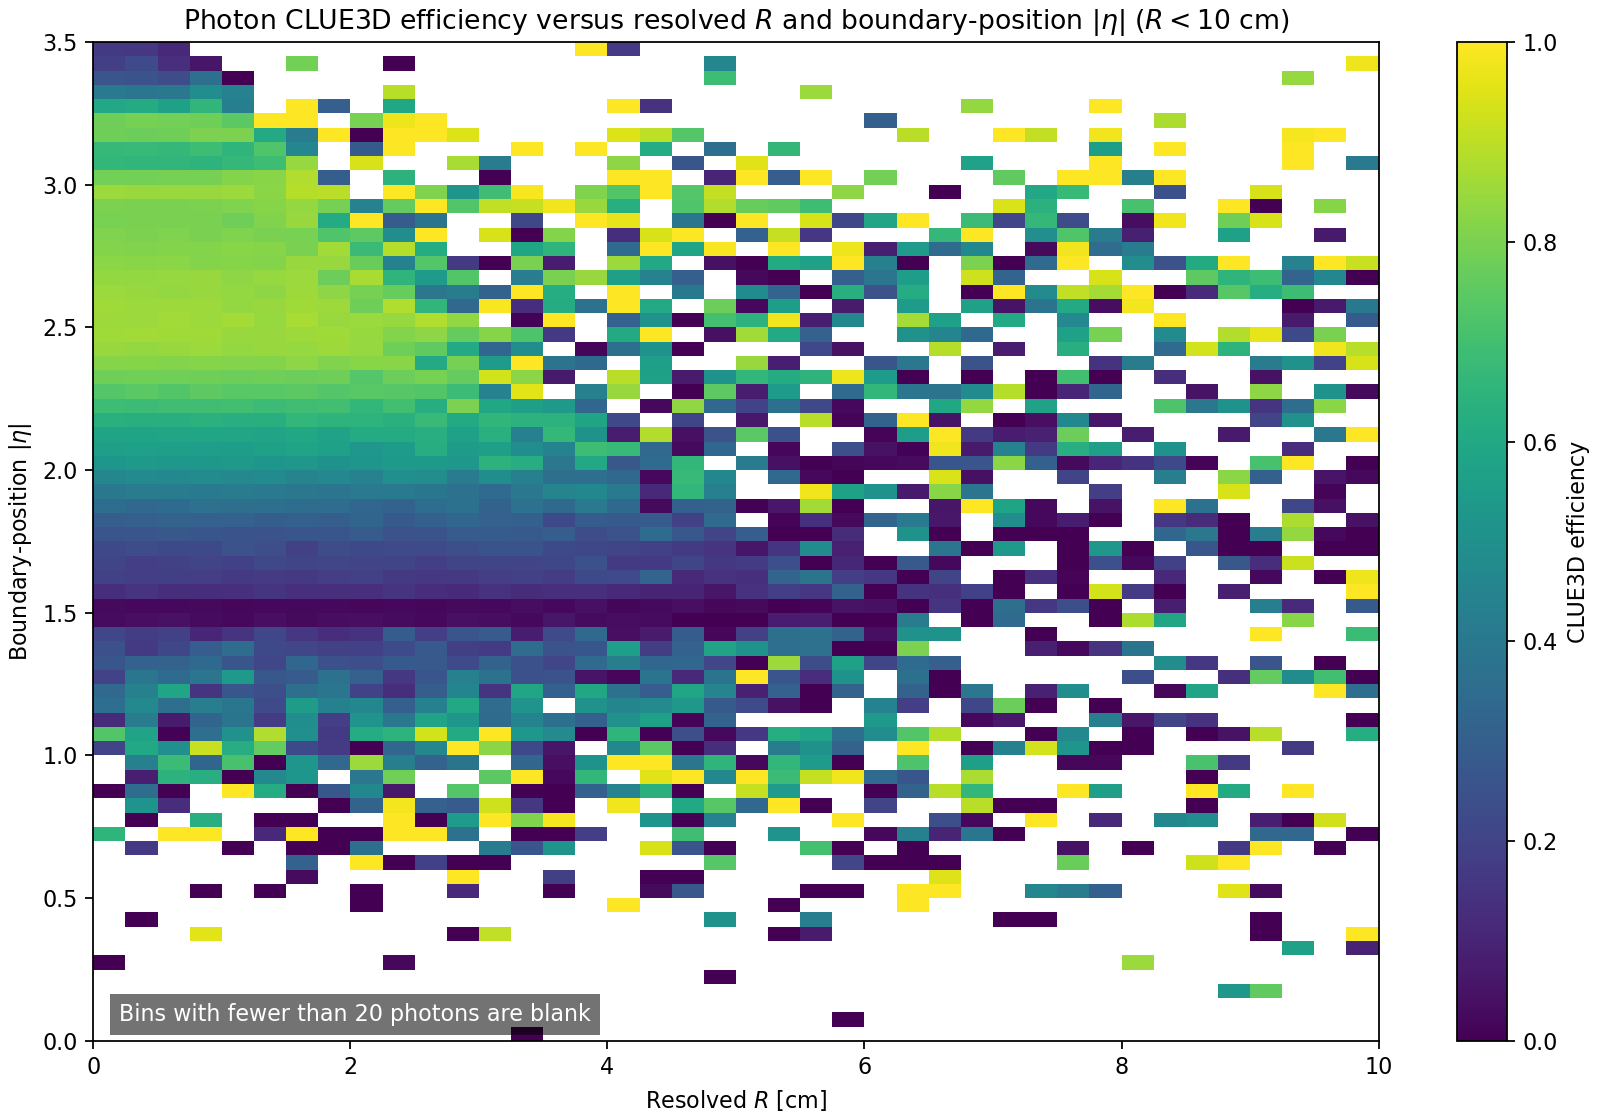
\includegraphics[width=\linewidth]{figures/pileup_photon_eta.png}
  \caption{Pileup-photon efficiency versus resolved $\R$ and boundary-position
  $|\eta|$ near the origin. Bins containing fewer than 20 photons are blank.
  The prominent angular structure motivates separating acceptance and
  kinematic effects from a dependence on displacement.}
  \label{fig:pileupphotoneta}
\end{figure}

For photons, the loss near the origin is concentrated in the low-energy
population, below about 2~GeV. The remaining dependence is really angular, not
on displacement. Pileup photons come from vertices close to the beamline, so
$z_v$ is small and Eq.~\eqref{eq:pileupphotonR} makes resolved
$\R=|z_v|\tan\theta$ essentially a proxy for the polar angle: a small increase
in $\R$ means a larger $\theta$ and hence a rapidly falling $|\eta|$. The
two-dimensional efficiency in Fig.~\ref{fig:pileupphotoneta} confirms this---the
structure runs in $|\eta|$ rather than in $\R$, with the loss confined to the
lower-$|\eta|$ edge of the HGCAL acceptance, where reconstruction is expected to
degrade. A
one-dimensional photon-versus-$\R$ curve therefore inherits this acceptance
edge and only looks like a displacement effect.

\subsection{Charged showers and LayerCluster multiplicity}

\begin{figure*}[!tp]
  \centering
  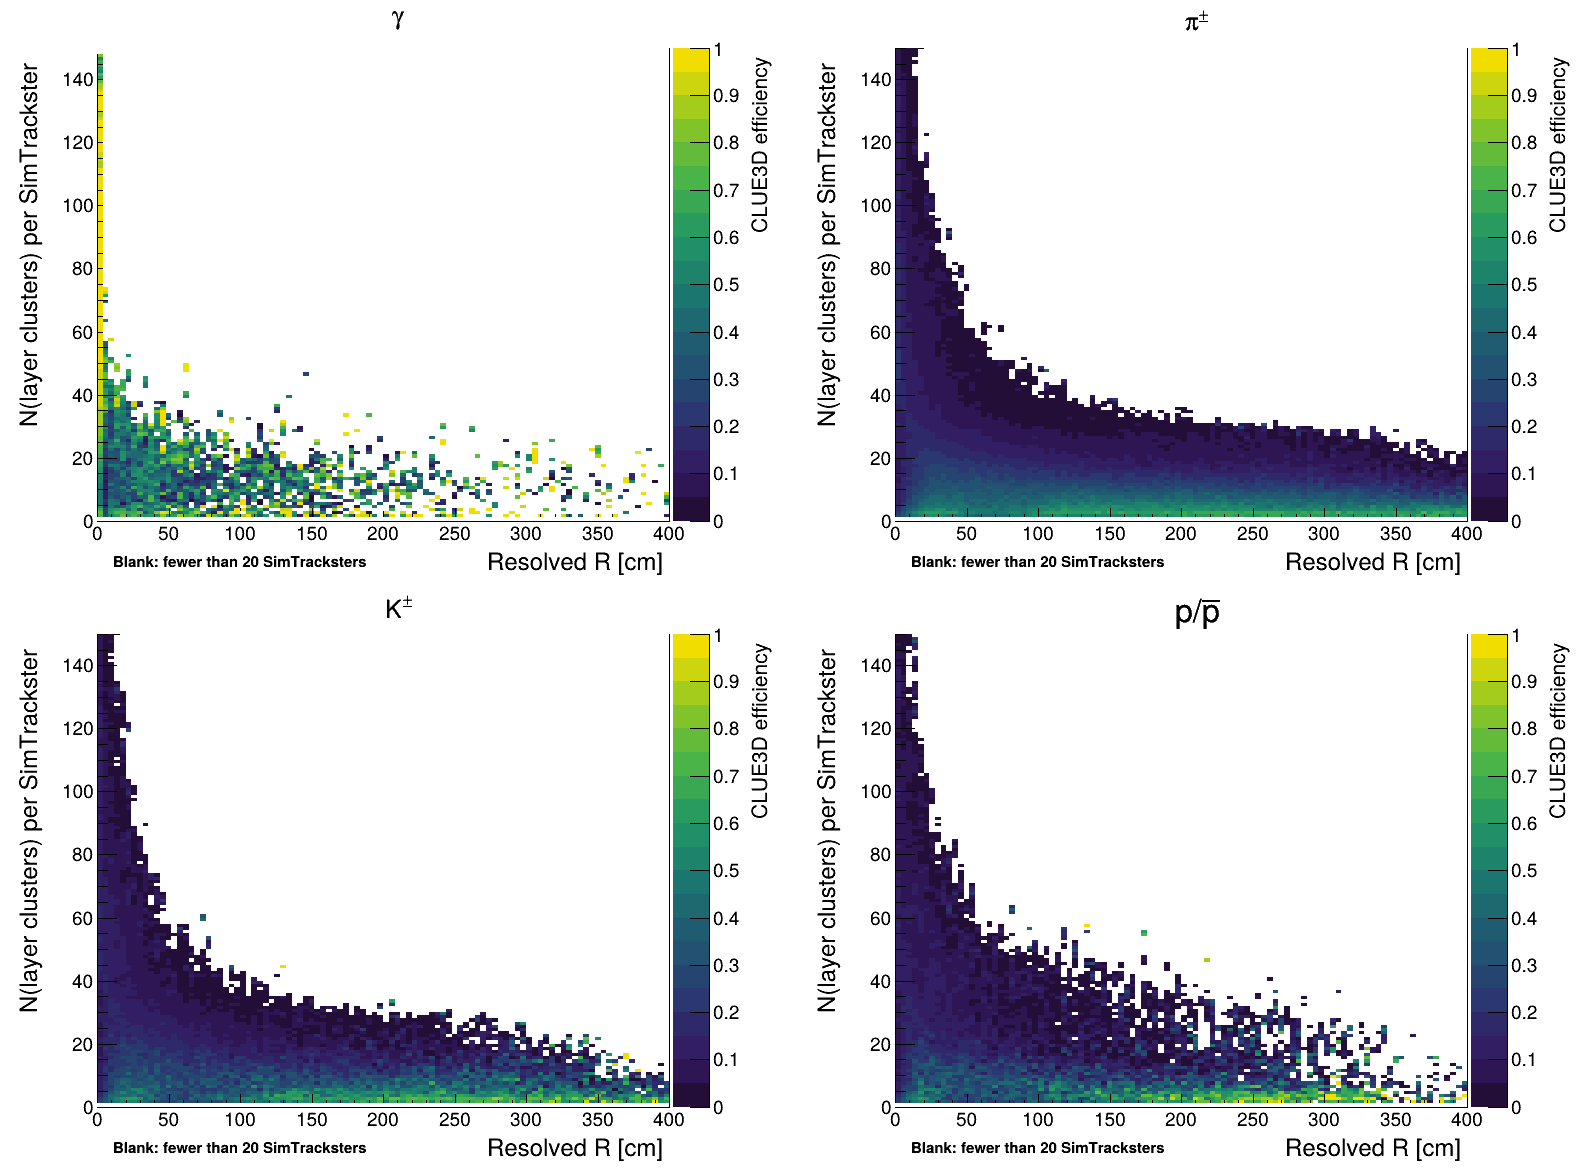
\includegraphics[width=0.9\textwidth]{figures/pileup_efficiency_lcs.png}
  \caption{Efficiency in bins of resolved $\R$ and truth-shower LC
  multiplicity, separated by particle species. The charged-hadron panels
  show lower efficiency for larger LC multiplicities and fewer large showers
  at large resolved $\R$. Blank bins contain fewer than 20 SimTracksters.}
  \label{fig:pileupshowersize}
\end{figure*}

For charged pions, kaons and protons the efficiency instead \emph{rises} with
resolved $\R$, the opposite of the photon trend, and the controlling variable
is the number of LCs in the truth shower: showers with many LCs rarely have
more than half of their energy collected in a single Trackster
(Fig.~\ref{fig:pileupshowersize}). As $\R$ grows, the whole pion
LC-multiplicity distribution shifts downward---not just its tail---so the
population moves towards smaller showers, and the charged-particle efficiency
rises with it.

Higher-momentum hadrons bend less, so they keep a smaller resolved intercept $\R$ while also developing
larger, higher-multiplicity showers; larger $\R$ therefore preferentially
selects the lower-energy, few-LC showers that \cluethreed{} reconstructs more
easily. This is a selection effect on the pileup population, not a direct
action of transverse displacement.

As an aside, similar connection first appeared the other way around. In
two-dimensional $(\R,\text{energy})$ and $(\R,|\eta|)$ efficiency maps for
pions, bins containing more reconstructed objects tended to have lower
efficiency. The natural guess was local crowding: that such showers sat in
busier neighbourhoods, where a high density of nearby reconstructed objects
might merge activity or otherwise disrupt the clustering. When I measured this
directly, however, efficiency showed no dependence on the number of
reconstructed objects in a shower's own neighbourhood, even at fixed $\R$,
energy and $|\eta|$.

Anyways, inclusive pileup efficiency must be
read together with particle identity, energy, angle and shower size, and the
signal-only selection remains the direct test of displaced-photon
reconstruction in pileup.
